
\begin{table}[h]
\centering
\vspace{-10pt}
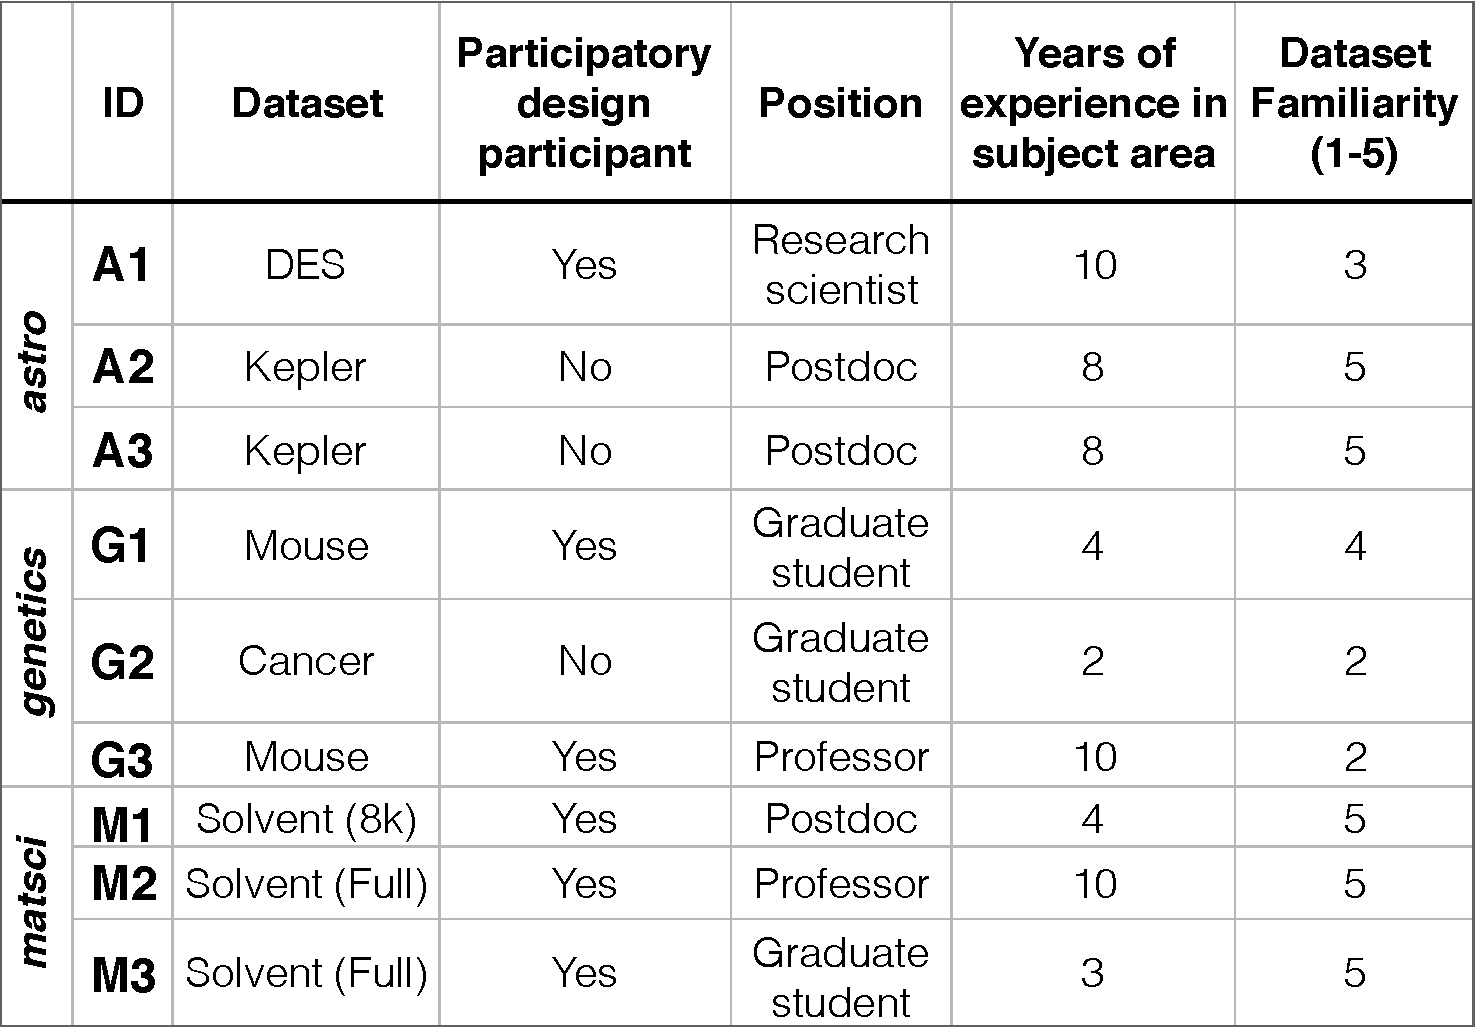
\includegraphics[width=\linewidth]{figures/participants.pdf}
\caption{Participant information. The Likert scale used for dataset familiarity ranges from 1 (not at all familiar) to 5 (extremely familiar).}
\label{participants}
\vspace{-10pt}
\end{table}

\par The research questions and objectives of the participants were diverse even among those in the same subject area and using the same dataset. Examples of research questions included: 
\begin{denselist}
\item Understanding gene expression profiles of breast cancer cells that exhibit induced, transient, and repressed patterns after a particular treatment.
\item Studying common patterns among stars that exhibit planetary transits versus stars that do not, from the Kepler space telescope\footnote{\url{www.nasa.gov/mission_pages/kepler/main/index.html}}.
\item Identifying battery solvents with favorable properties and mass production potential through studying how changes in certain chemical properties correlate with changes in other chemical properties. 
\end{denselist}

\begin{figure}[!h]
  \centering
  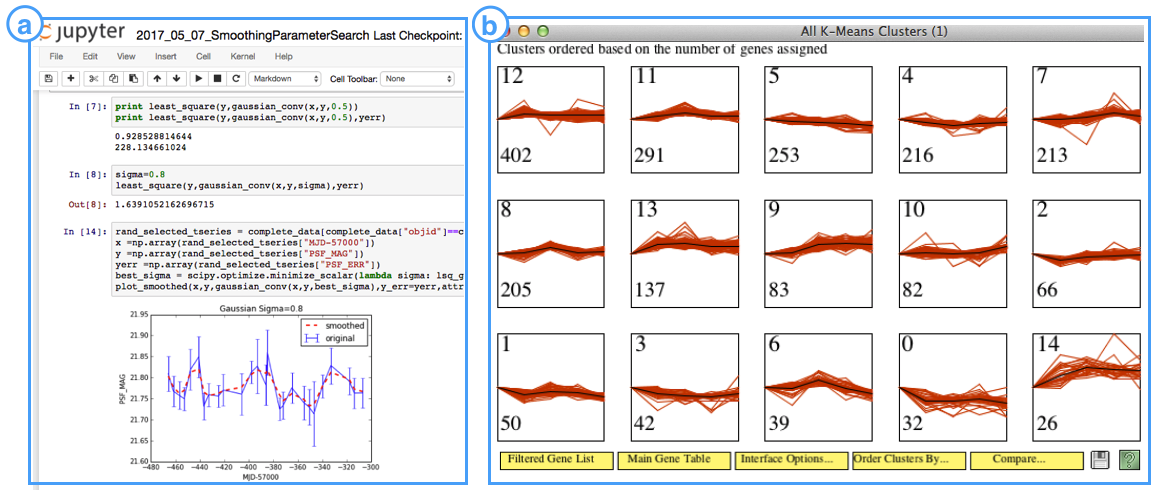
\includegraphics[width=\linewidth]{figures/workflow.png}
  \caption{Examples of the scientists' original workflow: a) The astronomer performs various data analysis task using the Jupyter notebook environment, b) The geneticists uses a domain-specific software to examine clustering outputs.}
  \label{workflow}
\end{figure}

\noindent The pre-study survey with the participants showed that out of all of the steps in their data analysis workflow\footnote{This includes viewing and browsing data, data cleaning and wrangling, computing statistics, data visualization, and model building or machine learning.}, they spend most of their time computing statistics and creating visualizations.
The main bottlenecks cited in their existing workflows included the challenge of dealing with large amounts of data, writing custom processing and analysis scripts, and long turnaround times incurred by making modifications to an upstream operation in a segmented workflow. %\ccut{On average, participants expressed interest in adopting \zv in their day-to-day workflow as eight from a Likert scale of ten after the study \kk{not sure what this means}.}
%%%%%%%%
 We  describe the three scientific use cases below.
